\chapter{Limitations \& Future Work}

\section{Limitations}

\textbf{Test Train Split Aggregation}

In some of the models, the test and train data are combined to normalise the data. This is to prevent data points in the test split with features larger than any data point in the test split exceeding a normalized value of 1. 

This is not correct as the train set should be isolated from the model during training.

While this does negatively impact the credibility of the evaluations of the models which have used this technique, the difference made is not likely to be significant enough to change the conclusions or future work in this project.

\textbf{Common Model Interface Removes Index}

The common model interface has been designed to prioritise integration between the NodeJS models and the scikit-learn models. Because both of these model types can read a CSV file, the interface is restricted to passing a CSV file path.

By passing a CSV file path, the DataFrame index is not kept. This blocks model12 from splitting a DataFrame, passing these splits to other models, and then reinserting the predictions into the same row the prediction came from.

Model12 therefore cannot be completed due to a limitation of the common model interface, a solution where the index is maintained would allow models of this type to be explored.

\textbf{Latitude \& Longitude Preprocessing}

Currently, the latitude and longitude preprocessing uses the centroids on the Unions only, not the Mouzas. This is because the function used to merge the geodata to the well data is unable to match the geodata Mouzas and the well data Mouzas, the reason why is not clear. 

With the Mouza centroids, higher resolution latitudes and longitudes could be provided to the models, allowing for more precise decision boundaries to be found.

\textbf{Further Analysis of Neural Network Models}
\label{fannm}

Further analyses of the neural networks will identify what their current limitations are and how they should be further developed to overcome these limitations.

Figure \ref{fig:x lc_m9} on page \pageref{fig:x lc_m9} shows the loss curve of model9 with 2 hidden layers of 50 nodes then 2 nodes. This shows that the decrease in loss is plateauing at 30 iterations, suggesting that further iterations will not provide a significant performance improvement. 

Figure \ref{fig:x lc_big_m9} on page \pageref{fig:x lc_big_m9} shows the sane neural network but with 3 layers of hidden nodes with 2000, 1000 and 100 nodes respectively. After 30 iterations, this model outperforms the model9 instance with less hidden nodes in terms of both performance and training loss. The tradeoff is more computational power being required, causing longer training and test time per iteration. 

The larger model, figure \ref{fig:x lc_big_m9}, is continuing to decrease loss by iteration 30. The larger model does however show signs of overfitting as the difference between the test and the train loss is increasing. This could potentially be mitigated with a larger validation split.  

This shows that more hidden nodes in the neural network produces better performance, though it has not been practical to test these models due to hardware limitations and time constraints.

\begin{figure}[!htb]
    \centering
    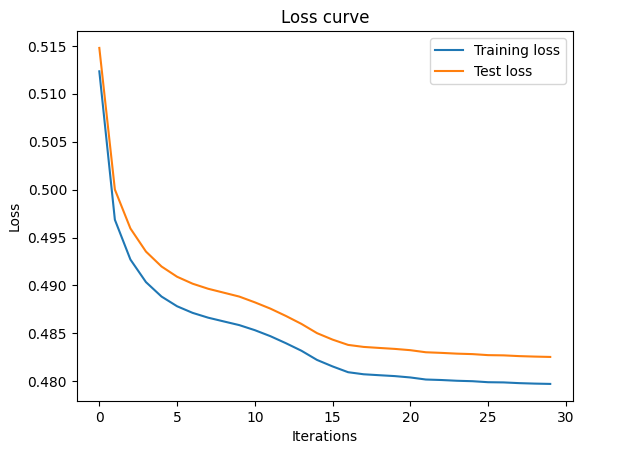
\includegraphics[scale=0.6]{figures/m9_loss_curve.png} 
    \caption{Model9 loss curve 50, 2 hidden layers}
    \label{fig:x lc_m9}
    
    \centering
    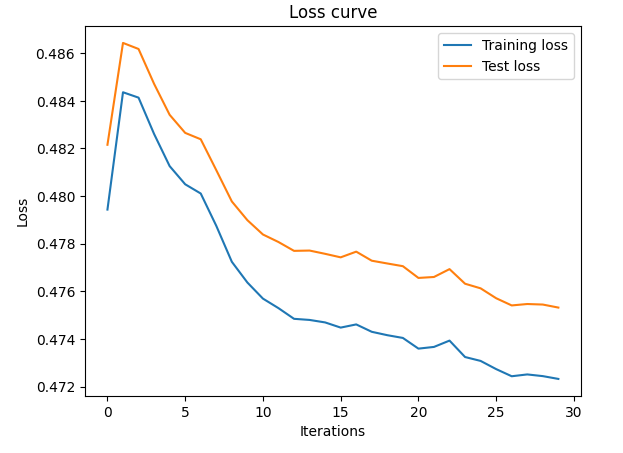
\includegraphics[scale=0.6]{figures/big_nn_loss_curve.png} 
    \caption{Model9 loss curve 2000, 1000, 100 hidden layers}
    \label{fig:x lc_big_m9}
\end{figure}

\section{Future Work}

\subsection{Further Data Integration}

\textbf{Flooding}

\cite{Connolly2022} states that flooding is a "key driver" of groundwater arsenic levels in southeast Asia. Preliminary investigations show that flooding data does exist, but is not readily available in a format which can be integrated into this project without significant preprocessing.

This preprocessing of available flooding data to produce a generic flooding data source could improve the performance of the iArsenic models, potentially achieving new performance records, or form the basis for new machine learning based models.

\textbf{River Geographic Data}

Polygon data for rivers in Bangladesh are readily available for download online. Because flooding tends to happen on riverbanks (see \cite{Connolly2022}), integrating river data into the existing models could be a convenient way to see if further work on higher quality flooding data will be worthwhile.

\textbf{Soil Parameters}

\cite{Winkel2008} shows data from the Food and Agriculture Organization of the United Nations correlates with groundwater arsenic pollution. Integrating this into the available data could allow new models to be trained or existing models to be improved.

\textbf{Elevation}

\cite{Connolly2022} excluded areas with slopes greater than 0.1 degrees from their model because arsenic pollution tends to occur in flat areas. Integrating this data would enable the optimization of the machine learning models, neural network based models in particular, as sloped regions could be ignored by the model.

\subsection{Different Model Types}

\textbf{Convolutional Neural Network Based Model}
\label{cnnbm}

In section \ref{fannm} on page \pageref{fannm} evidence is provided that the model9 neural network with the same design but more hidden nodes and layers perform better. But how many nodes and layers would be ideal?

There is no single rule for how many hidden nodes to use in a neural network, though in mode8, each layer uses half the number of neurons in the previous layer.

Following this rule, for 9,550 Mouzas, each with a latitude and longitude, the perfect network would have 19,100 input nodes (9,550 * 2) and 2 output nodes for a binary classification of 'safe' or 'polluted'. This would result in 12 hidden layers containing a total of 19,090 hidden nodes. This is an impossibly large neural network to implement.

This impossibly large design would allow the entire dataset to fit into the model without optimizing the dataset at the cost of key features.

With a convolutional neural network, these key features could be retained by passing one section of the dataset to the model at a time. The model could then identify patterns to look for within a radius of a data point's latitude and longitude instead of considering it in the context of the entire dataset. This should not impact performance as a data point is likely not dependent on far away data points.

The data is currently split by Division in model8 and depth strata in model14. These manual methods of splitting the data make assumptions about where decision boundaries should be, where a neural network should be able to identify these boundaries with training. Manually splitting the data also reduces the amount of data the model can learn from. Because a convolutional neural network would not require the data to be split into smaller datasets trained on multiple models, these disadvantages could be eliminated.

\textbf{Ensemble Model}

The Evaluation chapter shows that some models perform better than others, what is still not clear, however, is how often the best model outperforms the other models.

The plan for model12 is to take a training set, train and test every other model on the training set, see which model performs best for each region then pass data points in the test set to the model which performs best in that region.

A CSV of the best model for each Upazila can be see here at the following link, this data could not be used by an ensemble model however because this data has been generated from the test set: \url{https://github.com/JavaRip/UoP-SoftEng-Dissertation/blob/main/models/model12/best_model_by_upa.csv}

\textbf{Deep Learning Models \& Pruning}

Investigation of deep learning models has been designated outside the scope of this project. Features introduced by deep learning would allow for new model paradigms to be explored and reduce the negative impact on performance inflicted by current optimization techniques.

Neural network pruning for example could allow neural network models which convert regions to their latitude and longitude to work with higher precision and more detailed region sizes (Mouzas instead of Unions for example). 

Currently, an input node must exist for every point within a square which covers Bangladesh, including areas in neighbouring countries or the ocean. Implementing neural network pruning could allow these regions to be ignored by the model, instead of existing in the model to no benefit. The introduction of flooding, soil and evaluation parameters could also be aided by pruning.

\subsection{Further Development of iArsenic Models}

\textbf{Classification Threshold Manipulation}

The evaluation of the iArsenic models, and the machine learning models which required a common evaluation method, is limited by the inability to generate a receiver operator curve. This is because it is not possible to adjust the classification threshold of the iArsenic models. It would be possible to add this feature by changing the code in the iArsenic models.

\textbf{Future Work Detailed in iArsenic Repository}

The evaluation of the iArsenic models showed that they have increased in performance with each iteration. Further refinements to these models are detailed in the iArsenic repository so it is feasible that further iterations will garner further performance benefits.

\section{Conclusion}

There are four broad categories for future work, developing features to eliminate limitations, developing new models, integrating additional data and continuing development of the iArsenic models.

The most promising area of future development is the development of convolutional neural network models as this continues to expand on the research question, how do machine learning moels compare to the existing iArsenic models, by introducing further machine learning paradigms.